\chapter{Introduction} 

\section{Livestock farming, animal health and infectious diseases}

Livestock farming today is embedded in a complex socio-economic landscape that underpins food security, rural development, and environmental sustainability. As global populations rise and resource constraints become more acute, the ability to produce high-quality animal products in a sustainable manner is more critical than ever. This sector not only ensures the availability of nutritious food but also supports the livelihoods of countless rural communities, thereby reinforcing local economies. In parallel, the modern challenges of animal health and public safety are converging, with infectious diseases emerging as a significant threat that jeopardizes both the productivity of farming systems and the broader public health framework. The traditional approach to livestock management, which often treats animal health in isolation, is increasingly being questioned in favor of a more integrated strategy that acknowledges the intricate links between animal welfare, human well-being, and environmental health—a perspective encapsulated by the “One Welfare” paradigm.

In this context, infectious diseases are not merely biological phenomena but are embedded within the socio-economic fabric of livestock farming. Their impact reverberates through production losses, escalating veterinary expenses, and the overuse of antibiotics, which in turn contribute to public health concerns such as antimicrobial resistance. These challenges demand a rethinking of conventional control measures and underscore the urgency of developing sustainable farming practices that can adapt to both immediate crises and long-term environmental pressures. By embracing an integrated approach, the sector can transform these challenges into opportunities for innovation, leveraging advanced technologies and interdisciplinary strategies to enhance animal health, protect public well-being, and ensure the economic viability of farming systems for future generations.

This section provides a comprehensive overview of the socio-economic landscape that surrounds livestock farming, underscoring its importance for food security, public health, environmental management, and the integrated “One Welfare” approach. It section also highlights key challenges related to the impact of infectious diseases on livestock farming as well as conventional methods used to diagnose, manage, and prevent these diseases and their inherent limitations.

\subsection{Socio-economical context and the stakes}



% Finally, the rationale for integrating new, data-driven modelling approaches is introduced, emphasizing their potential to improve disease surveillance and decision-making. These methods aim to complement the expertise of farmers and veterinarians by providing more accurate prognostics, optimizing resource use, and ultimately contributing to more resilient and welfare-focused livestock farming systems.

\subsubsection{Livestock Farming, animal health well-being}



First, we define the core concepts:
\begin{itemize}
    \item Livestock Farming: The organized breeding and raising of animals for food, fiber, and other products.
    \item Animal Health and Well-Being: The physical and psychological state of animals, which directly impacts productivity and the quality of the products.
    \item Sustainable/Self-Sufficient Livestock Farming: Farming systems that are designed to maintain productivity and animal health over the long term with minimal reliance on external inputs, promoting environmental, economic, and social resilience.
\end{itemize}

[remarks: Approfondis la notion de bien-être animal et de santé publique.
Souligne l’importance des approches intégrées comme celle recommendé pour le "One welfare" pour montrer comment la santé animale, la santé humaine et la préservation de l’environnement sont étroitement liées et prennent de plus en plus de place la société d'aujourd'hui et à venir. ]

Next, we examine why sustainable livestock farming is critical in today’s global context:

\begin{itemize}
    \item Food Security: As the global population grows, the demand for high-quality animal products increases. Ensuring that farming practices are sustainable helps guarantee that future generations will have access to sufficient, nutritious food. This involves not only meeting quantity demands but also maintaining quality standards.
    \item Animal Welfare and public Health: The safety of the food supply is paramount. Sustainable practices reduce the risks of diseases that can be transmitted between animals and humans. Maintaining robust animal health also minimizes the use of interventions, such as antibiotics, which can lead to issues like antibiotic resistance.
    \item Environmental and Ecological Management: Livestock farming significantly contributes to environmental challenges such as greenhouse gas emissions, pollution, and deforestation. Transitioning to sustainable systems can mitigate these impacts, balancing food production with the need to preserve natural ecosystems.
    \item Resource Management: Efficient farming requires the optimal use of resources—land, water, energy, and labor. Sustainable systems are designed to reduce waste and improve efficiency. This is particularly important as both the availability of resources and the demand for skilled labor (veterinarians, farmers, technicians) face increasing pressures in many parts of the world.
\end{itemize}

By addressing these interrelated aspects, sustainable livestock farming not only tackles immediate socio-economic challenges but also contributes to long-term ecological balance and public health protection.


\subsubsection{Infectious diseases - impact on livestock farming}

[remarks: Donne quelques références bibliographiques pour illustrer la fréquence de certaines maladies (les plus connues sauf les BRD) dans différents contextes (régions géographiques, modes d’élevage intensif/extensif).]



Infectious diseases are disorders caused by pathogenic microorganisms—such as bacteria, viruses, fungi, that can spread directly or indirectly from one host to another. These diseases can manifest across different domains, affecting both humans and animals, and their transmission may occur at multiple scales—from within a single host to entire metapopulations.

\textbf{Types and Transmission Patterns:} Infectious diseases vary by type. For instance, respiratory infections (e.g., COVID-19 in humans and certain respiratory illnesses in animals) and sexually transmitted diseases (such as AIDS in humans) illustrate the diversity of these conditions. In the animal domain, examples like African swine fever and bovine viral diarrhea underscore how pathogens can devastate livestock. Some infections are zoonotic, meaning they can jump from wildlife to livestock and even to humans (E.g., Ebola, monkeypox), highlighting the interconnectedness of human, animal, and environmental health. Transmission can occur in several ways, including host-to-host contact, within-host dynamics, and across populations, which sometimes creates complex patterns that pose significant public health challenges.

The effects of infectious diseases are far-reaching:
\begin{itemize}
    \item Ecological impact: Inappropriate or excessive use of antimicrobials in response to infections can lead to the emergence of resistant bacteria. This resistance not only renders certain treatments ineffective but also complicates recovery, thereby jeopardizing both animal and human health.
    \item Food Safety and Security: Outbreaks can cause major production losses in livestock farming by reducing both the quality and quantity of animal products. These losses threaten the broader goal of achieving food security, especially in regions where livestock is a primary source of nutrition and income
    \item Animal Health and Welfare: Infectious diseases directly compromise the health and well-being of animals, leading to suffering and significant economic losses for farmers.
    \item Resource Management: Managing infectious diseases demands frequent monitoring and diagnosis, along with substantial investments in vaccines, antibiotics, and veterinary expertise. This imposes a heavy financial and operational burden on farming systems, making sustainable practices even more challenging to implement.
\end{itemize}

By understanding these aspects, one recognizes that controlling infectious diseases is not only a matter of public health but also a critical component of creating sustainable and self-sufficient livestock farming systems.

\textit{\textbf{Keywords:}} infectious diseases, critical concern, animal welfare, animal health, antimicrobial resistance, economical loss, production loss, food safety, public health, epidemiology

% Did I miss key ideas that could help me demonstrate why infectious diseases in livestock farming are interresting topics in society currently ? 
% Also i think inn this subsection i need to give more example of infectious diseases in the livestok farming context. The other ones (for humans, or wild animals) are juste to give an idea or illustrate something. 

\subsection{Conventional control strategies of infectious diseases}
\label{Conventional control strategies} % ajout-du-label-pour-faire-reference-a-la-sous-section


[remarks: Donne plus de détails sur les stratégies de contrôle et de prévention]
[remarks: Pour la partie sur la détection et la gestion classiques (examen clinique, analyses de laboratoire), enrichis avec un cas d’usage : comment se déroule une journée de surveillance dans une ferme, comment l’éleveur travaille-t-il avec le vétérinaire ?]

[remarks: Parle des défis de surveillance épidémiologique à grande échelle (temps, coûts, organisation).]

\subsubsection{Diagnose, prognose and recommend control measures}

Effective management of infectious diseases in livestock relies on a systematic process that begins with accurate diagnosis, proceeds with reliable prognosis, and culminates in tailored recommendations for control measures. Each step is crucial for mitigating outbreaks and ensuring the long-term sustainability of farming systems.

\paragraph{Diagnosis.} The first step involves identifying the presence and nature of the disease. Diagnosis can be achieved through:
\begin{itemize}
    \item Clinical Appraisal: This is the most common method among farmers, where visual or tactile observations are used to detect clinical signs in animals. While this approach is quick and accessible, it is inherently subjective and may lead to inconsistent interpretations.
    \item Biological Examinations: In this approach, samples such as blood or mucus are collected for laboratory analysis (e.g., PCR testing). Although this method can provide a more precise identification of pathogens, it is often more invasive, time-consuming, and may delay decision-making during fast-moving outbreaks.
\end{itemize}

\paragraph{Prognosis.} Once the disease is diagnosed, the next step is to forecast its progression and potential impact. Prognosis typically relies on:
\begin{itemize}
    \item Expert Knowledge: Veterinarians draw on empirical observations and scientific experimentations (detail more how they build knowledge pieces by pieces) knowledge, to predict the disease trajectory.
    \item Historical Data: Farmer can also rely on past events and past decision outcomes to help inform the likely spread of the disease. 
    % though variability between farms or over time can challenge generalization and accuracy.
\end{itemize}

\paragraph{Recommendation of Control Measures.} Based on the diagnostic and prognostic assessments, appropriate control measures can be devised. These measures are intended to:
\begin{itemize}
    \item Reduce the spread of the disease within and between farms.
    \item Minimize production losses and safeguard food safety.
    \item Optimize the use of resources such as veterinary expertise, time, and financial investment.
    \item Balance short-term emergency responses with long-term sustainable practices
\end{itemize}

While these conventional methods have proven useful, they come with inherent limitations.

\textit{\textbf{Keywords:}} Diagnosis, clinical appraisal, biological examinations, prognosis, expert knowledge, empirical observations, scientific experimentations, recommendations, control measures.


\subsubsection{Challenges to tackle}

\paragraph{Limitations in Diagnosis:} 
\begin{itemize}
    \item Subjectivity and Inconsistency: Visual and manual examinations by farmers or experts, though common, are inherently subjective. Different observers may interpret clinical signs in various ways, leading to inconsistent diagnoses.
    \item Scalability Issues: Manual diagnosis becomes increasingly impractical as farm sizes grow or when frequent assessments are necessary. This limitation is critical as rising demand requires more rapid and consistent monitoring.
    \item Intrusiveness and Delay in Biological Testing: Biological examinations (e.g., blood sampling and PCR testing) offer greater precision but are invasive and time-consuming. The time lag in obtaining results can allow the disease to progress before control measures are implemented.
\end{itemize}

Challenges in Prognosis:
\begin{itemize}
    \item Limited Expertise and Resource Constraints: Relying on expert judgment for prognosis is not scalable. The shortage of veterinarians, especially in rural areas, exacerbates the challenge of providing timely and accurate prognoses across large populations.
\end{itemize}

Addressing these challenges is essential for enhancing the reliability and scalability of disease management strategies. 


[remarks, lien avec la section suivante: Évoque les solutions émergentes comme l'IA. Évoque le rôle de la modélisation ]





[l’utilisation de capteurs (température, rythme respiratoire), de bases de données partagées ou encore de méthodes d’apprentissage automatique.]

\textit{\textbf{Keywords:}} subjectivity, scalability, shortage of expertise, costly, laborious, time-consuming, animal stress, repetitive

% il faudrait que je trouve un endroit où mettre les défifintiosn de certains mots: metapopulation par exemple ?  mais c'est mieux de l'insérer dans le texte si c'est facilemetn possible. 
% je peux jeter un coup d'oel sur l'article de pauline pour avoir d'autres argument
% et regrader de le docs de maud si on parle de méthode traditionnele de control des maladies infectieuse: éleveur comme vétos.
% je vais devoir chercher les chiffres pour argumenter certains faits. example: ethical concerns...

% my old notes
% - il faut bien préciser que c'est ce qui est le plus répandu car c'est le minimum et c'est à la portée de tous mais elle a également ces limites.
% - observation des eleveurs et des experts
% - estimation des états de santé ... 
% - doses des traitement non adaptés: phénomène de resistance des bactéries
% - la santé animale qui prend chère
% - méthode purement empiique qui mais qui peut couter chère
% - d'un environnement à l'autre ce n'est pas toujours les mêmes stratégies qui peuvent être appliquées
% - scalable ? update of the knowledge ? transferability to other issues ? 
% - manual job that is not consistant but it is the baseline that has always been done
% - le problème c'est que non seuelemnt les eleveurs seuls ne possèdent pas toute la connaissance véto et/ou de modélisateurs pour optimiser de manière rigoureuse et stable les .... (lire l'article de pualine pour prouver pourqoui cees méthodes ne peuvent pas faire long terme tel quels s'ils ne sont pas automatisé. (ils ne sont pas mauvais, mais iil faut une pratique standardisé)

% - conclure sur la self-suffisiancy ou susbtainability des filières par rapport aux maladies respiratoires. 
% - Tacler tous ces problèmes nécessites la mise en place de méthodes qui sont repoductible, compréhensible/interpretable, facilement utilisable, et qui sont construit en impliquant la connaissances des tous les acteurs de la filière concernées. 

% - L'idéée est d'avoir des méthodes qui peuvent aider à aléger la tâche aux éleveurs afin qu'ils consacrent leur energies, argent, temps et efforts sur des problèmes à plus forte valeur ajoutés.  
% peuvent nous aider à mimer et faire mieux ou de manière fiable ce ce qu'on.

%----------------------------------------------------------------------------------------
%	SECTION 
%----------------------------------------------------------------------------------------
\clearpage 


\section{Artificial intelligence}

[Insère un court paragraphe sur la manière dont la modélisation (épidémiologique, statistique ou via l’IA) peut aider à affiner les pronostics et à améliorer la prise de décision.

Même si tu détailleras cela plus tard dans la thèse, indique déjà les perspectives que cela ouvre pour optimiser la prévention et le contrôle des maladies respiratoires. ]

Artificial intelligence (AI) has its roots in early attempts to formalize logical reasoning and problem solving through symbolic systems, a period often referred to as 'Good Old Fashion AI' (Nilsson, 2009; Russell \& Norvig, 2010). Over time, the field evolved dramatically, particularly with the advent of machine learning, in which algorithms learn patterns directly from data instead of relying on explicitly encoded rules (Mitchell, 1997; Goodfellow et al., 2016). Within machine learning, deep learning has emerged as a major paradigm, leveraging large, multilayered neural networks to address complex, high-dimensional tasks such as image classification and speech recognition (LeCun et al., 2015).
Despite the success of these data-driven methods, the AI systems commonly encountered in mainstream applications, such as virtual assistants or image-tagging services, represent only one slice of a broader ecosystem. In particular, epidemiological modeling provides a knowledge-driven complement, capturing essential mechanisms of disease transmission and population dynamics (Keeling \& Rohani, 2008; Allen, 2017). While deep learning excels at recognizing patterns in raw data, epidemiological models integrate biological or domain-specific insights, offering interpretability and the ability to extrapolate beyond training distributions.
Bringing these perspectives together can give rise to hybrid solutions that combine the strengths of data-oriented learning and mechanistic reasoning (Childs et al., 2019; Wang et al., 2021). Such integrated approaches have the potential to enhance both predictive accuracy and robustness, particularly in complex domains such as livestock disease management.
This section begins by presenting an overview of precision agriculture and the sensors that collect the core data required for AI applications in farming contexts. It then discusses stochastic mechanistic models, highlighting how they capture disease dynamics, along with their typical challenges and limitations. Next, the focus shifts to deep learning, addressing both its remarkable performance in pattern recognition and its known constraints, such as interpretability and sensitivity to data shifts. Finally, the section explores how hybrid strategies can reconcile the benefits of mechanistic epidemiological approaches with the pattern-detection capabilities of deep learning, laying the groundwork for more effective modeling of respiratory diseases in livestock.

\subsection{Precision agriculture: hardware and sensors}

Precision agriculture represents an innovative approach to farming that focuses on optimizing inputs (such as feed, medication, and energy) while maximizing outputs, including net profit and environmental sustainability. This paradigm is rapidly being adopted in livestock farming to enhance decision-making and operational efficiency. At its core, precision agriculture is supported by a robust infrastructure consisting of both hardware and software components. In this subsection, we concentrate on the sensors that underpin data collection:


\begin{itemize}
    \item Behavioural Data: For instance, accelerometers can record movement patterns of individual animals.
    \item Positional Data: Electronic identification systems (such as Eartags) track animal locations and movement across the farm.
    \item Biological Data: Devices like intraruminal boluses can continuously monitor physiological metrics such as body temperature.
    \item Environmental Data: Connected sensors measure ambient conditions, such as temperature and humidity, which can influence animal health.
    \item Operational Data: Information regarding feeding schedules and management practices can also be recorded to provide a comprehensive picture of the farming environment.
\end{itemize}

One of the major benefits of these sensors is their configurability. They can be tailored to collect data at various spatial scales—from detailed individual observations to broader herd-level trends—and temporal resolutions, whether through continuous real-time monitoring or periodic measurements. This scalability ensures that both micro-level behaviours and macro-level patterns are captured effectively. 

By leveraging these advanced sensor systems, precision agriculture can provide a more objective, scalable, and comprehensive means of monitoring livestock health, thereby addressing some of the inherent limitations of conventional observational methods.

Although sensors deliver raw observational data that is closely linked to the emergence and spread of infectious diseases, a conceptual gap remains. The challenge lies in processing this unstructured, multi-dimensional data to extract meaningful insights and translate them into actionable recommendations.

\textit{\textbf{Keywords:}} sensors, automated data collection, multi-modal datasets, scalable, customizable.

% if you have more examples of sensors used in precision agriculture, then i shoudl insert it here. I don't want to mention anyy modelling strategies here nor do i want to mention any, just want to stay limited on the sensors and hardware so do you have any more ideas ? 

\subsection{Epidemiological modelling: Stochastic mechanistic models}

Epidemiological models serve as valuable tools for understanding, predicting, and controlling the spread of infectious diseases. By combining theoretical knowledge of disease transmission dynamics with empirical observations, these models provide insights that guide public health and veterinary interventions.

\paragraph{Fundamental Concepts and Historical Context.} Epidemiological modelling has deep roots in classical infectious disease research, with early examples focusing on simple compartmental models (e.g., SIR, SEIR). Over time, these models have evolved to capture more nuanced disease dynamics and real-world complexities. They explicitly represent the biological and ecological processes governing infection spread, such as contact rates, recovery patterns, and immunity mechanisms. By embedding domain knowledge, mechanistic models are interpretable and allow researchers to dissect how various factors influence disease trajectories.

\paragraph{Stochastic Mechanistic Models.} Stochastic approaches extend mechanistic models by incorporating random events—such as unpredictable contact opportunities, mutations, or interventions—thereby accounting for variability in disease spread. Key features include granular representation of uncertainty (Randomness in infection times and transmission events is captured, leading to a range of possible outcomes rather than a single deterministic trajectory). Stochastic models can better handle heterogeneous populations (e.g., different farms, varying animal susceptibility), especially when data are limited or events are sporadic. Scenario Exploration : Researchers can run multiple simulations under different assumptions or interventions, providing valuable insights into potential disease outcomes without requiring large-scale, real-world experimentation.

Interpretability and Biological Realism: By embedding expert knowledge and explicit mechanisms, these models help highlight the interactions and feedback loops that drive disease progression.

Hypothesis Testing and Policy Guidance: Stochastic mechanistic models allow for the evaluation of “what-if” scenarios, enabling more informed decisions on control measures—such as vaccination strategies or biosecurity protocols.

Although powerful, stochastic mechanistic models can become mathematically complex.

\textit{\textbf{Keywords:}} epidemiological stochastic mechanistic models, explicit representation of underlying mechanisms, incorporation of as much knowledge as we want, explainable predictions and insights, evidence-based recommendations, extrapolation


\subsubsection{Identifiability and observability}

Identifiability and observability are fundamental concepts in epidemiological modelling and statistical inference. They describe our ability to determine meaningful information about a system based solely on available observations (relire l'article de nik cunniffe et frederic hamelin)

Identifiability: Refers to whether the parameters of a model can be uniquely and accurately estimated from the available observations. In epidemiological modelling, a model is identifiable if different parameter values always lead to distinct observational outcomes. A lack of identifiability implies multiple plausible explanations exist for the same observed data, making reliable inference difficult.

Observability: Closely related to identifiability, observability refers specifically to the possibility of inferring the internal state of a system from available observations. An observable epidemiological model allows researchers to infer hidden states (e.g., the number of infected or susceptible animals at a given time) from external observations (e.g., clinical signs, ultrasound imaging, sensor data).

The challenges of identifiability and observability are central when modelling livestock diseases, as they directly affect the reliability of predictions, diagnoses, and recommended interventions. When parameters in a mechanistic epidemiological model cannot be reliably identified, the predictions become uncertain, undermining effective disease management.

Challenges of using epidemiological mechanistic models in Livestock farming:

\begin{itemize}
    \item Parameter inference, conversely, aims to estimate model parameters directly from context-specific observational data. It typically provides more precise results tailored to the studied population or outbreak but requires sufficient data quantity and quality, as well as more computational resources and advanced inferential methods. Real-world epidemiological models often have many parameters. As model complexity increases, the parameter space grows exponentially, a phenomenon known as the "curse of dimensionality." This makes it increasingly difficult to accurately infer parameters from observational data, especially when the quantity or quality of data is limited. 
    \item Manual Processing and Scalability Issues: often, methods including visual analysis or expert-driven parameter selection, are time-consuming and hard to scale. Manual identification of observable patterns or features from raw data becomes impractical when dealing with extensive datasets, particularly data derived from videos, audio recordings, or continuous sensor measurements. Livestock observational data, such as ultrasound imaging or audio recordings of animal coughs, often contain high levels of noise and unstructured information. Such data are challenging to interpretate even by experts, severely limiting scalability and accuracy.
\end{itemize}

\textit{\textbf{Keywords:}} Parameter identification, fitting to non-structured observations, differentiating models, manual model fitting does not scale-up.

Even thought these modelling approach are arguably the best to study and control complex diseases, they still have a few but critical challenges to be tackled. Being able to exploit their knowledge on non-structure observations (which are very frequent in the real-world) would also make them more widely used. 


\subsection{Machine learning modelling: Deep learning models}
Machine learning is a subfield of artificial intelligence involving algorithms that allow computers to learn patterns or relationships directly from data. The defining characteristic of machine learning models is their ability to improve their predictive performance through exposure to increasing amounts of data, rather than through explicitly programmed instructions. Within machine learning, deep learning models represent a sophisticated subclass, specifically designed to handle complex, high-dimensional, and unstructured data. Deep learning employs artificial neural networks—computational models inspired by biological neural systems—which consist of interconnected processing units called neurons arranged in layered architectures. This hierarchical structure enables deep learning models to learn intricate data representations at multiple abstraction levels.

In this thesis, we give extra attention to deep learning architectures, for their high performance in data-mining, pattern extraction in unstructured data which are an efficient format for storing high dimensions observations in their closest form to the original state: "one image contains a thousand words". 
Deep learning models are exceptionally powerful in tasks requiring automatic pattern extraction, and they are frequently described as universal approximators, capable of capturing non-linear relationships and subtle features from large and varied datasets. Typical examples include:

\begin{itemize}
    \item Image classification: Identifying objects or diseases from medical or veterinary images (e.g., ultrasound images).
    \item Natural language processing (NLP): Understanding and generating human language, such as sentiment analysis and text classification.
    \item Speech recognition: Automatically transcribing spoken audio signals.
\end{itemize}

There are methods implemented to enhance the explainability of deep learning models (XAI):
\begin{itemize}
    \item Grad-Cam and LIME produce saliency maps. They provide visual explanations by highlighting important regions of an input image that contribute to a neural network's prediction. Grad-CAM is specific to convolutional neural networks (CNNs) and generates heatmaps by computing gradients of the predicted class score relative to the CNN's intermediate convolutional layers, emphasizing regions that strongly influence the prediction. In contrast, LIME is model-agnostic, working by creating local perturbations around the input data, fitting a simple interpretable model (such as a linear regression) to approximate the behaviour of the original model, and highlighting input regions that most significantly affect the prediction. They are several other methods, such as DeepLIFT (Deep Learning Important Features, SmoothGrad, occlusion sensitivity). 
    \item Uncertainty quantification such as Bayesian deep learning or conformal predictions. There is no rivalry. They are radically different frameworks achieving very different things. CP is about calibrating predictions, while the Bayesian framework is about quantifying uncertainty of various things from the model, parameters, and consequently, the predictions. The typical guarantee you get from the Bayesian framework is that your estimates/predictions achieve the smallest average loss over the prior. That means Bayesian estimators are optimal estimators in terms of average performance, meaning they will be accurate, but do not guarantee coverage. CP does nothing about the accuracy of your estimator but gives you coverage. You can combine both and have the best of both worlds. One can understand this from a PAC-Bayesian perspective: CP is related to the empirical risk, while BDL is related to the KL divergence between the posterior and prior. 
\end{itemize}

These examples illustrate the flexibility and adaptability of deep learning across multiple application domains, including precision agriculture and epidemiological diagnostics. Despite their remarkable capabilities, deep learning models present certain limitations critical in epidemiological and livestock farming contexts. 

\textit{\textbf{Keywords:}} Deep learning, automated pattern extraction, handles unstructured observation, most powerful function approximator, intrapolation, uncertainty quantification, XAI


\subsubsection{Limitations and Challenges of classical Deep Learning Models}

% Interpolative vs extrapolative knowledge

Deep learning methods typically assume the data to be independently and identically distributed (iid), meaning each data point is generated from the same probability distribution and independently from one another. Deviations from this assumption can significantly degrade model performance and generalization capabilities.

% \begin{itemize}
%     \item Lack of Interpretability and Biophysical Meaning: Deep learning models are often described as "black-box" models due to their complexity and limited interpretability. The learned parameters (weights and biases) generally do not possess direct biological or mechanistic meaning, making it difficult to understand why a model produces a certain prediction.
%     \item Overfitting and Generalization: With high capacity and flexibility comes the risk of overfitting, where the model learns dataset-specific noise or irrelevant patterns rather than meaningful generalizable trends. Consequently, achieving robust generalization performance beyond the training set can be challenging.
%     \item Requirement for Extensive and Representative Data: Deep learning models rely heavily on datasets that comprehensively represent the underlying phenomena of interest. Insufficient or biased training data can lead to suboptimal generalization, especially in disease diagnostics, where precise and representative datasets are rare, difficult to collect, or ethically challenging to generate (e.g., intentionally inducing disease outbreaks).
%     \item Sensitivity to Distribution Shifts (Out-of-Distribution Data): Deep learning models typically struggle when encountering data outside their training distribution (Out-of-Distribution, OOD). This limitation is particularly pertinent in epidemiology, where the appearance of previously unobserved disease variants or changes in environmental conditions frequently occur.
%     \item these methods can also quickly become very resource intensive particularly when dealing with complex task as often the architecture also get more complex, requiring bigger infrastructure (gpu, cpu) for training or inference, these also has an impact on environmental management.
% \end{itemize}

XAI methods are a way to measure and understand why predictions are made, They are usually are employed for outliers detection, data drift, ...  however they cannot be used to precisely forecast extreme scenarios. 

Each of these methodologies individually addresses certain specific aspects of infectious disease modelling effectively, but they also carry inherent limitations when applied alone:
\begin{itemize}
    \item Deep learning models excel at extracting intricate patterns from large-scale or high-dimensional observational data (e.g., sensor-derived data such as audio, video, or biological signals). Their data-driven nature allows them to effectively capture context-specific and complex relationships without explicit theoretical assumptions. Nevertheless, their main limitation lies in their lack of explicit biological or theoretical interpretability, limiting their capability to reliably extrapolate to unseen scenarios or out-of-distribution contexts.
    \item Stochastic mechanistic epidemiological models explicitly encode theoretical or biological mechanisms (infection transmission, recovery rates, or disease progression) using interpretable parameters with clearly defined biological meanings. These models can thus generate hypotheses, facilitate understanding of causal dynamics, and provide robust extrapolation to scenarios not explicitly observed in the data. However, their main challenge lies in effectively incorporating detailed, unstructured, and context-specific observational data (such as sensor data), limiting their practical utility and responsiveness to specific epidemiological contexts.
\end{itemize}

% Even thought these model are widely used to process complex datasets, they are hardly used to explore novel situations or predict task that are inherently has multiple complex relationships (so hard to gather a representative dataset). these challenges essentially stem from the lack of explicit knowledge incorporation (example hallucinations in LLMs). They are in their need of feature that could  enhance interpretability, improve generalization in OOD settings, and facilitate more accurate and meaningful insights by explicitly incorporating domain-specific knowledge into the learning process.


% do models like PINN require more data ? 
% otherwise the advantage of what we are proposing will be on the structure i guess. A modular method, that could require a bit less since we are training a a less complex task. at yet maybe as performant ? 

% prmireè formulation: a methodology that can be used to process non-structure datasets and still easily be used to extrapolate towards unknown complex scenarios.
% second thing incorporate more knowledge into the observation that are gathered because sometimes the observations are noisy and don't represent the global mechanisms. 

\textit{\textbf{Keywords:}} Generalization, forecast extreme scenarios, input dataset has to be iid, lack of biophysical meaning of parameters, black-box modelling, data intensive for complex tasks, resource intensive (GPU, electricity, materials...) for complex tasks, false positive, false negative, extrapolation


\subsection{Hybrid modelling: machine learning and epidemiological models}

[Raccourci cette partie pour garder le tableau, le plus important c'est de montrer les objectifs (summarize), les types de couplages (summarize), montrer les axes que nous mettons en avant]
En terme d'objectif voici les cases que nous cochons: model parameterizination, disease intervention assessemnt and optimization, restrospective epidemic course analysis, infectious disease forecasting (par contre préciser qu'ici en réalité nous avons n'avons pas fait de forecast dans le sens statistique du terme jusqu'à aller à l'évaluation des performances, transmission inference, outbreak detection]

[Résumé les objectifs en un paragraphe. Etendre par contre le type de d'intégration et comment c'est fait. mettre égalemenet le rôle que joue chaque partie ?] [the roles are long-term forecast (or prognose) or short-term predictions]

This section serves as a concise narrative review of various methodologies for integrating machine learning models with epidemiological models, offering a critical perspective on their limitations. Addressing these limitations is central to the contributions of this thesis.

This section presumes that the reader possesses a foundational understanding of ensemble techniques in modelling, specifically bagging, boosting, and stacking. They are pivotal in enhancing the global performance by combining multiple models. These methods aim to reduce errors, improve accuracy, and increase the robustness of predictions. Stacking Combines outputs from several distinct models using an additional "meta-model," learning optimal combinations for improved predictions. Boosting refers to sequentially training multiple weak predictive models, each aiming to correct errors from previous models, thus progressively improving overall prediction accuracy. Bagging (or Bootstrap Aggregating) refers to parallel training of multiple unique models (while stacking used distinct models, bagging uses multiple instances but of the same model) on random subsets of data (with replacement), thereby reducing prediction variance and mitigating over-fitting.

In the scientific literature, hybrid modelling approaches integrating deep learning and mechanistic models have gained attention, especially during epidemiological crises such as the COVID-19 pandemic. Several prominent methodologies in this domain include:

En sciences, toute tentative de tirer des conclusions généralisables nécessite un
modèle, i.e. une version abstraite de la réalité \cite{McCallum2008}. Cette représentation
abstraite est dotée d’un objectif (a model is a "purposeful representation", 
\cite{Starfield1990}, qui requiert un certain degré de simplification.

The purposes of the hybrid models currently found in the litterature can be grouped into 6 mutually exclusive groups, indicating that a single integrated model serve multiple application areas \cite{Ye2025} :
\begin{itemize}
    \item Infectious disease forecasting: Predicting the future spread or trajectory of infectious diseases by combining AI's data-mining strengths with the explanatory power of mechanistic epidemiological models. 
    \item Model Parameterization and Calibration: Determining and refining model parameters (e.g., disease transmissibility, contact rates) accurately and efficiently, often by extracting additional insights from diverse and complex datasets.
    \item Disease Intervention Assessment and Optimization: Evaluating and identifying optimal strategies for interventions (such as vaccinations, social distancing, or lockdowns) to minimize disease spread and impact, utilizing methods like reinforcement learning and game theory. 
    \item Retrospective Epidemic Course Analysis: Understanding past epidemics by analyzing historical data, identifying critical factors influencing transmission dynamics, and informing future outbreak preparedness.
    \item Transmission Inference: Inferring hidden patterns, source origins, and transmission networks using AI techniques trained on data from mechanistic epidemiological simulations or real-world data.
    \item Outbreak Detection:Quickly identifying new outbreaks or unusual surges in cases, enabling timely public health responses through AI-enhanced analysis of varied data sources, such as medical reports or social media content.
\end{itemize}


Methodologicaly-wise, these models can also grouped into nine primary integration approach:

\textcolor{red}{Rajouter également une colonne pour le indiqué le format des données (textes, image, videos, audio) - simulées/vrai - et colonne pour le problème (covid, ...)  à rajouter dans la colonnes training process (texte..., simulés) et objective (covid...)}
 Peux-être regrouper les colonnes intregration approach et citations pour gagner de l'espace. (dimuner) aussi les marges.

\begin{center}
\begin{longtable}{|p{3cm}|p{3cm}|p{3cm}|p{3cm}|p{3cm}|}
\caption{Summary of nine primary integration method types.}
\label{tab:integration_methods} \\ 
\hline
\textbf{Integration approach} & \textbf{Objectives} & \textbf{Description} & \textbf{Training process} & \textbf{Original citations} \\ 
\hline 
\endfirsthead

\multicolumn{5}{c}%
{{\bfseries \tablename\ \thetable{} — continued from previous page}} \\ 
\hline
\textbf{Integration approach} & \textbf{Objectives} & \textbf{Description} & \textbf{Training process} & \textbf{Original citations} \\ 
\hline 
\endhead

\hline \multicolumn{5}{r}{{Continued on next page}} \\ \hline
\endfoot

\hline
\endlastfoot
    
Learning Unknown Components of Epidemiological Models (e.g., PINNs, EAAMs, Synthetically‐trained AI models) & Incorporate time‐varying dynamics and diverse datasets for parameter inference and forecasting. & AI models are used to “learn” unknown components (such as state variables, parameters, or derivatives) within mechanistic models by embedding epidemiological principles (e.g., via residual loss terms) into the network architecture. & End‐to‐end supervised training using gradient‐based optimization (e.g., Adam or SGD) on real or synthetic datasets. & References \cite{kharazmi_identifiability_2021, barmparis_physicsinformed_2022, de_rosa_modelling_2023, torku_seinn_2023,berkhahn_physics-informed_2022, rodriguez_einns_2023, shaier_data-driven_2022, bertaglia_asymptotic-preserving_2022, malinzi_determining_2022} for PINNs; \cite{liu_rolling_2023, otadi_universal_2017, liu_epidemiology-aware_2023, amini_mepognn_2023, sun_2022, gao_stan_2021, zheng_spatial-temporal_2021, ma_enhancing_2022, wang_causalgnn_2022, nguyen_becaked_2022, nguyen_becaked_2022-1} for EAAMs;  \cite{wang_tdefsi_2020, zhan_optimizing_2021, wang_deep_2021, bogacsovics_replacing_2021, wang_predicting_2022, murphy_deep_2021, zhang_understanding_2021, quilodran-casas_digital_2022, silva_data_2022} for synthetically‐trained models \\ \hline


Training AI Models Using Synthetic Data & Leverage simulated epidemiological data to uncover disease transmission patterns. & Mechanistic models are used to generate synthetic datasets under varying parameter conditions; AI models (e.g., RNNs) are then trained on these datasets to predict unknown model components or future epidemic trajectories. & Supervised learning on synthetic datasets using standard optimization methods. & References \cite{petrica_inverse_2023,liu_prediction_2023,rahnsch_network-based_2024,kumar_epidemic_2023,ji_climate-dependent_2023,vega_simlr_2022,chen_covid-19_2023,alsmadi_susceptible_2023,qiu_prediction_2022,mu_modelling_2023,wang_machine_2021,wu_computer_2022,yao_assessment_2022,zhang_prediction_2021,wyss_modeling_2023,gadewadikar_methodology_2024,zisad_integrated_2021,merkelbach_hybridml_2022,munoz_hybrid_2022,castillo_ossa_hybrid_2021,jiang_countrywide_2021,yasami_application_2022,liao_sirvd-dl_2021,zheng_predicting_2020,watson_pandemic_2021,liu_nesting_2023,wang_policy_2022,wang_hypothesis-free_2022,deng_dynamics_2020,kim_determination_2021,gupta_deep-siqrv_2023,bousquet_deep_2022,feng_data_2022,ding_biology-informed_2023,khan_attention_2022,kumaresan_analysis_2022,long_identification_2021} \\ \hline

Embedding Epidemiological Knowledge into AI Models & Enhance model plausibility by enforcing epidemiological constraints. & Domain knowledge (e.g., conservation laws or differential equations governing disease spread) is integrated into the AI model’s inputs, loss functions, or architecture, ensuring that predictions adhere to known epidemic dynamics. & Custom loss functions combining data fit with epidemiological residuals are minimized via gradient-based optimization. & See Supplementary Appendix 16 and related studies (e.g., \cite{kharazmi_identifiability_2021,barmparis_physicsinformed_2022,de_rosa_modelling_2023,torku_seinn_2023,berkhahn_physics-informed_2022,rodriguez_einns_2023,shaier_data-driven_2022,bertaglia_asymptotic-preserving_2022,malinzi_determining_2022}) \\ \hline

Optimal Decision-Making via AI Models (Reinforcement Learning & Optimal Control & Identify optimal intervention strategies in dynamic epidemic settings. & AI frameworks—using reinforcement learning or optimal control—leverage simulations from mechanistic models to determine time‐dependent control actions (e.g., intervention policies) that balance disease and socioeconomic outcomes. RL agents are trained within epidemiologically based environments or neural networks approximate control variables, using iterative optimization techniques. & References \cite{yao_optimal_2023,zou_data-efficient_2021,vereshchaka_optimization_2021,song_reinforced_2020,probert_context_2019,ohi_exploring_2020,khadilkar_optimising_2020,hao_reinforcement_2022,libin_deep_2021,awasthi_vacsim_2022,song_robust_2023,padmanabhan_reinforcement_2021,kompella_reinforcement_2020,mai_planning_2023,asikis_neural_2022,roy_knowledge_2021,colas_epidemioptim_2021,capobianco_agent-based_2021,ou_active_2021,trad_towards_2022,bushaj_simulation-deep_2022,chadi_2022 ,guo_pacar_2022,kulkarni_optimizing_2022,deng_optimal_2021,hwang_optimal_2022,wan_multi-objective_2022,miralles-pechuan_methodology_2020,bampa_epidrlearn_2022,shami_economic_2022,du_district-coupled_2022,benalcazar_deep_2021,xia_controlling_2022,khatami_reinforcement_2021,zong_reinforcement_2022,du_hrl4ec_2023,nguyen_general_2022,beigi_application_2021} for RL methods; \cite{yin_optimal_2023,asikis_neural_2022,courtes_reduced_2024,li_robust_2021,kmet_neural_2023,kmet_bezier_2019} for optimal control frameworks \\ \hline

Enhancing Observational Data & Improve the quality of surveillance data used for model calibration. & AI techniques extract auxiliary information from non‐traditional sources (such as social media, search trends, or emergency reports) to augment and refine conventional epidemiological datasets. & Supervised learning using classifiers (e.g., SVMs, tree-based methods) to infer health status and generate enhanced observational datasets. & References \cite{tuarob_modeling_2015,solares-hernandez_adaptation_2023,rosato_extracting_2023,kandula_improved_2019}\\ \hline

Ensemble Modelling of AI and Epidemiological Models & Boost forecasting accuracy by combining diverse model outputs. & Predictions from both AI and mechanistic models are aggregated using ensemble techniques (e.g., weighted averaging, stacking, or boosting) to produce more robust epidemic forecasts. & Individual models are trained separately and then combined—often with a meta-model (such as an LSTM-based stacker) trained on historical performance—to optimize forecast accuracy. & References \cite{kandula_evaluation_2018,adiga_all_2021,nadler_neural_2020,maniamfu_lstm-based_2023,adiga_enhancing_2022,delli_compagni_hybrid_2022}
\\ \hline

Clustering-Based Decomposition of Epidemiological Models & Decompose large-scale models for localized and more manageable analysis. & Clustering methods (e.g., k-means) are used to partition populations or regions into groups with similar epidemic characteristics, enabling tailored analysis and intervention evaluation. & Unsupervised clustering algorithms are applied to epidemiological data, with subsequent validation using agent-based or compartmental modelling approaches. & Reference \cite{bertozzi-villa_archetypes_2023} \\ \hline

\end{longtable}
\end{center}

% \end{tabular}%
% }
% \caption{Summary of nine primary integration method types.}
% \label{tab:integration_methods}
% \end{table}


\newpage


\begin{itemize}
    \item Physics-Informed Neural Networks (PINNs): PINNs integrate known governing equations (e.g., differential equations describing infectious dynamics) as soft constraints into neural networks during training. The neural network is guided by both observed data and theoretical knowledge, ensuring physically plausible predictions and improved extrapolation beyond the training distribution.
    \item Neural Differential Equations (Neural ODEs/SDEs): Neural ODEs or SDEs embed neural networks into differential equations, allowing the modelling of dynamic processes through continuous-time representations. Such integration directly captures temporal dynamics, offering more flexibility and interpretability compared to classical discrete-time deep learning methods.
\end{itemize}

% Despite their promising advantages, hybrid and ensemble models have inherent challenges:
% Despite notable advancement in the scientific community, there is a conceptual gap, between the raw unstructured livestock data that can be captured and the strong theoretical knowledge we have of the complex underlying infectious mechanisms. This basically allows to ground the theoretical knowledge we have on a complex mechanisms to the context-specific observations, hence harness the best of both world. 

\begin{figure}
  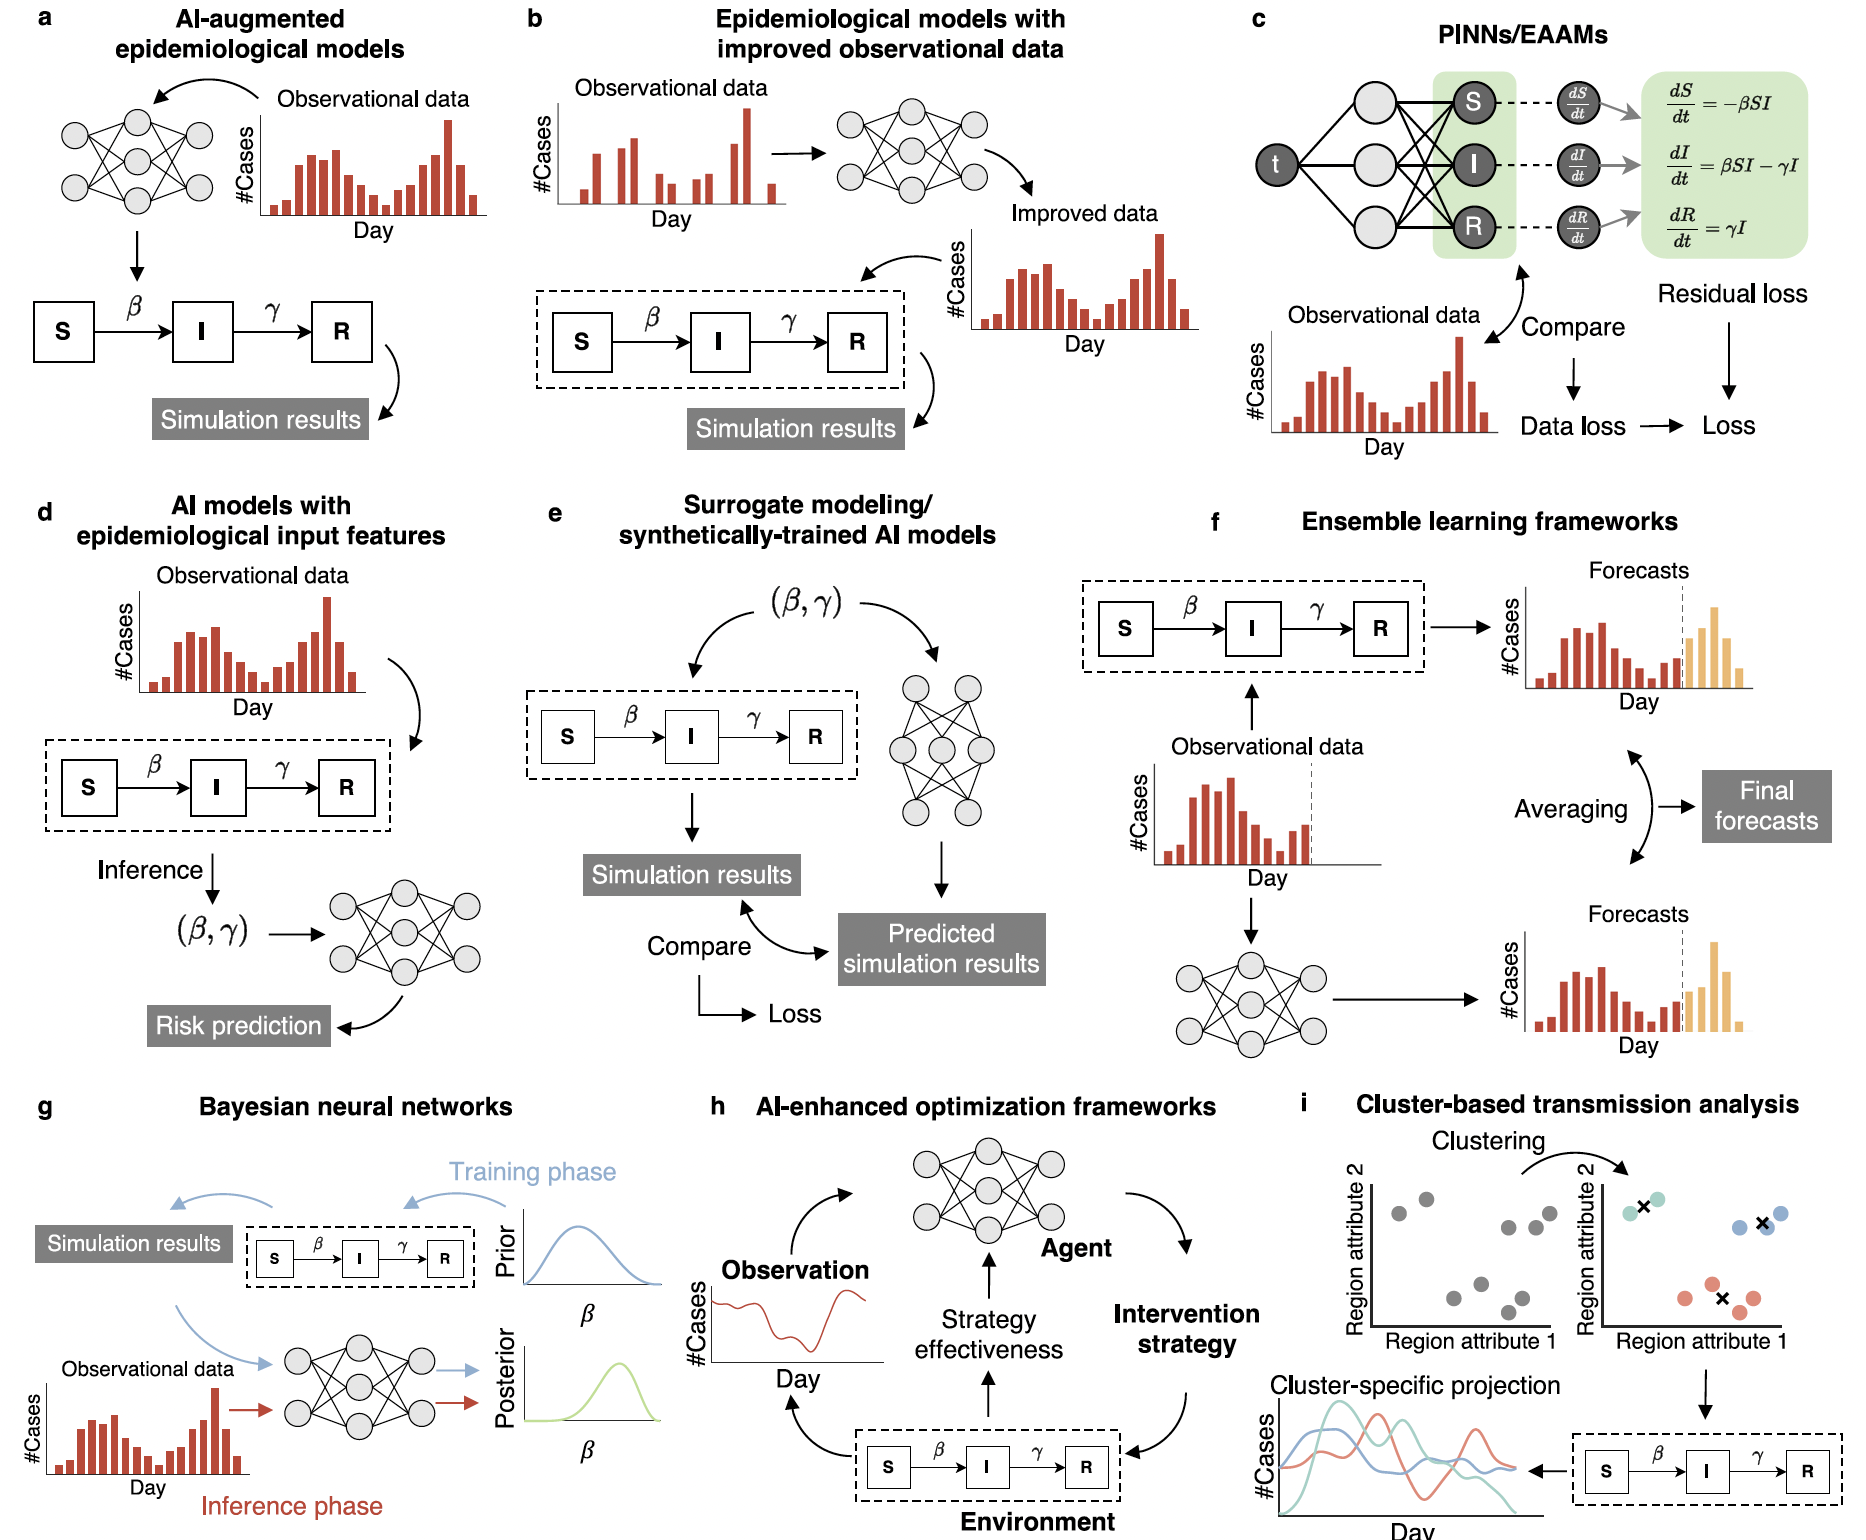
\includegraphics[width=\linewidth]{figures/chap1/chap1-hybrid.png}
  \caption{Illustrative examples of methodological frameworks coupling Machine learning (AI) and epidemiological models}
  \label{fig:chap1-hybrid}
\end{figure}



\textit{\textbf{Keywords:}} Ensemble learning, Physics-informed neural networks, Neural differential equations


% Each ensemble strategy presents specific strengths and limitations, related to computational complexity, interpretability, and predictive power. 
% research gaps:
% \begin{itemize}
%     \item Generalizability: The majority of integrated models focus on diseases like COVID-19, limiting applicability to other infectious diseases with indirect or complex transmission routes.
%     \item Expansion beyond COVID-19 to other diseases with indirect transmission mechanisms.
%     \item Data Limitations: Many studies depend on synthetic or limited real-world data, highlighting the need for richer, real-time data integration (e.g., satellite imagery, social media data). - we have gathered in this thesis a real-wolrd multi-modal dataset (...)
% \end{itemize}

% je vais enlever cette subsub section, elle ne sert à rien
% \subsubsection*{Maintainability}

%     \begin{itemize}
%         \item strongly coupled methods requires the builder to be deeply understand the problematic of domain in order to implement the models. (full stack vs frontend or backend). So retraining for example would require the whole system to be trained and in the long-term, it would also require sort of full-stack builders. 
        
%         \item strongly coupled methods would still require a  certain quantity of data since in order for example for the deep learning model to fine-tune the mechanistic model (neural differential equations). Usually ensembled model (so more parameters) would require more dimensions in order to fit all the parameters (curse of dimensionality)
%     \end{itemize}

% le domaine est très large, mais nous on va se focaliser uniquement sur le couplage deep et modèle méchaniste de façon générale. 

% sachant que nous c'est une forme de boosting, sans trop de redondances,) et surtout découplé (faiblement couplé) - ceci sont des couplages forts mais comme un site web à egalement ces limites. comme un développeur full stack - parler rapidement des NDE, des pinns qui sont juste une sous familles des NDE.



%----------------------------------------------------------------------------------------
%	SECTION 
%----------------------------------------------------------------------------------------
\clearpage 

\section{Thesis objective and outline}

\subsection{Exploring the complementarities between deep learning and mechanistic epidemiological models}

Precision agriculture provides powerful tools enabling automation of real-world observations through various sensors. Throughout this thesis, we have leveraged such tools to acquire contextual observational data essential for studying an infectious disease in livestock farming. However, sensor-based observations, although rich and increasingly accessible, represent only partial information regarding complex and unpredictable disease dynamics, aptly summarized by Yoan Bourhis (2017): "Nos observations ne révèlent que la partie émergée d’un iceberg au comportement complexe et peu prévisible."

Thus, a central question guiding this thesis is: How can sensor observations be effectively employed to study infectious diseases and support informed decision-making?

Our main hypothesis is that the most scientifically robust approach to contemporary quantitative questions in animal health, particularly regarding livestock infectious diseases, lies in combining complementary artificial intelligence methods, specifically deep learning and mechanistic epidemiological models. Such integration leverages deep learning’s capabilities for processing and extracting short-term insights from unstructured (video, image or text) observations  and the extrapolative capacities of stochastic epidemiological models grounded in explicit theoretical knowledge for long-term insights. This combination aims to better link real-world observations obtained through sensors with our theoretical knowledge in order make make relevant evidence-based recommendations at a larger temporal scales.

This naturally raises another foundational question addressed in this thesis:
In what ways can deep learning complement mechanistic epidemiological models in epidemiology ?

Complex animal health problems, including the study and control of infectious diseases, require distinct yet interconnected types of expertise: diagnosing diseases from immediate observational data, making reliable prognoses about future disease dynamics, and ultimately providing actionable recommendations. Diagnosis relies predominantly on processing unstructured field observations from sensors—thus favouring deep learning. Robust prognosis, however, relies on explicit theoretical knowledge and interpretability—domains inherently suited to mechanistic models. Finally, the quality of actionable recommendations is critically dependent on effectively bridging these two forms of expertise.

This thesis proposes a loosely coupled methodology inspired by the statistical principle known as the "Mixture of Experts" (MoE). This modular integration allows each expert to specialize explicitly in its distinct role (diagnosis and prognosis), enhancing accuracy, resource efficiency, interpretability, and scalability.

Addressing these considerations, the scientific questions explored throughout this thesis are:

\begin{enumerate}
    \item To what extent can deep learning reliably automate short-term diagnosis using limited, noisy, and context-specific observational data from sensors, such as lung ultrasounds ? 
    
    \item How can mechanistic epidemiological models be reliably parametrized using empirical veterinary observations to provide accurate long-term prognosis for infectious diseases ?
    
    % \item Given multiple mechanistic epidemiological models validly representing different expertise symptomatic dynamics of infectious diseases, how can observational data alone reliably guide the selection of the most appropriate mechanistic model to enable pathogen-specific disease management ?
    
    % \item How can observational data alone guide the selection of the best mechanistic prognosis expert when they are multiple epidemiological models expert for expliciting different mechanisms of the infectious disease.
    
    \item Given multiple mechanistic epidemiological models representing different but valid expertise in prognosing an outbreak, how can observational data alone reliably guide the selection of the most appropriate mechanistic model to enable pathogen-specific disease management.

    \item How can deep learning and mechanistic models be effectively integrated into a hybrid diagnostic-to-prognostic pipeline that leverages their complementary strengths to improve livestock disease management ?
    
    \item How can uncertainties inherent in sensor-based observations be explicitly accounted for within a hybrid modelling approach, and how does this influence diagnostic and prognostic reliability ?
\end{enumerate}


\textit{\textbf{Keywords:}} methodological synergy, complementary expertise, deep learning, mechanistic epidemiological models, diagnostic accuracy, prognostic reliability, uncertainty quantification, Mixture of Experts, modular architecture, scalability.

\subsection{Application to study Bovine Respiratory Diseases}
% In this subsection, I want to show that BRD are a good example for the application of our methodology

Bovine Respiratory Diseases (BRD) refer to a group of complex, multifactorial infectious disorders predominantly affecting young cattle in fattening farms. They are characterized by inflammation of the respiratory tract, causing symptoms such as cough, nasal discharge, fever, reduced feed intake, impaired growth, and occasionally, death. Although several pathogens (viruses, bacteria, mycoplasma) contribute to BRD, their clinical presentation is frequently non-specific, complicating accurate and timely diagnosis.

Diagnosing and managing BRD effectively remains notoriously challenging for several reasons:
\begin{itemize}
    \item Non-specific Clinical Signs: Clinical manifestations of BRD (e.g., cough, fever) are highly unspecific and overlap significantly with other diseases. Consequently, visual appraisal by farmers and veterinarians often results in misdiagnoses or delayed diagnoses, leading to suboptimal treatment strategies.
    \item Limitations of Biological Diagnostic Methods: Laboratory methods (e.g., Polymerase Chain Reaction (PCR), serology) provide increased specificity and accuracy compared to clinical appraisal alone. However, these tests are invasive, expensive, and time-consuming, delaying actionable results and increasing animal stress and discomfort. Moreover, logistical issues frequently limit their practicality, especially in large-scale operations.
    \item False Positives and Diagnostic Uncertainty: Due to the multifactorial nature of BRD (co-infections, pathogen interactions, host susceptibility variability), diagnostic and prognostic accuracy remain challenging. These difficulties result in inappropriate usage of antimicrobials, contributing to the rising threat of antimicrobial resistance and negatively impacting animal welfare.
\end{itemize}

(Complexity of BRD Etiology) BRD arises from complex interactions between intrinsic and extrinsic factors:
\begin{itemize}
    \item Pathogen Diversity and Interactions: Multiple pathogens (e.g., Mannheimia haemolytica, Pasteurella multocida, Bovine Respiratory Syncytial Virus, etc.) are frequently involved, potentially interacting in complex and poorly understood ways. Current veterinary research continues to explore these interactions to better characterize clinical markers useful for early detection, prognosis, and improved control measures (as exemplified in recent doctoral works, e.g., Maud’s research).
    \item Influence of Environmental and Management Practices: External factors such as farm management, biosecurity measures, herd density, transportation stress, and climatic conditions profoundly influence the occurrence and severity of BRD outbreaks. This intrinsic and extrinsic complexity significantly complicates disease modelling, prognosis, and control efforts.
\end{itemize}


(Socioeconomic Impact of BRD in Livestock Farming) Bovine Respiratory Diseases represent a major health and economic burden for farmers, veterinarians, and the broader livestock industry:
\begin{itemize}
    \item Economic Costs and Mortality Rates: BRD accounts for substantial economic losses in terms of reduced growth performance, increased mortality rates, and heightened veterinary and medicinal expenses. Particularly in French beef fattening farms, BRD is considered one of the most prevalent and economically significant animal health problems.
    \item Antimicrobial Usage and Ethical Concerns: Frequent misdiagnosis or delayed interventions lead to inappropriate use of antibiotics, fostering antimicrobial resistance. This concern raises ethical, public health, and animal welfare issues and highlights the urgent need for improved diagnostics and targeted therapeutic approaches.
\end{itemize}

(Existing Technological Approaches and Limitations) Recent research has applied sensor technologies (e.g., intra-ruminal temperature sensors, accelerometers, audio and video analytics) coupled with traditional machine learning and deep learning methods to improve BRD detection. Although promising, these data-driven approaches often:
\begin{itemize}
    \item Exhibit high false-positive rates due to limited specificity in clinical signs or ambiguous sensor outputs.
    \item Require substantial volumes of training data to achieve reliable performance, a constraint given practical difficulties in generating extensive labelled datasets.
    \item Struggle to predict disease progression or forecast epidemiological outcomes accurately over extended periods, thus limiting their use in proactive disease management and intervention strategies.
    \item Lack the capability to explore unobservable scenarios, such as hypothetical outbreaks or unrecorded infections, limiting their utility for scenario-based disease control planning.
\end{itemize}

There are also been mechanistic models developed before and throughout this thesis to model and study BRD (see Originality of this thesis). They have never applied to real-world observations. In this thesis, we employed these models to assess our methodology.

By bridging sophisticated deep learning feature extraction with robust, interpretable mechanistic models, this hybrid approach could significantly advance the ability to manage BRD effectively—improving animal health, welfare, farm economics, and sustainability and ecological issues. 

This thesis leverages BRD as a scientifically significant case study to validate a hybrid deep-mechanistic methodology, explicitly addressing the limitations noted above, with the aim of substantially improving diagnosis, prognosis, and disease management strategies in livestock farming.

\textit{\textbf{Keywords:}} Bovine Respiratory Disease, infectious disease dynamics, antimicrobial resistance, multi-modal data integration, predictive analytics, animal welfare.


\subsection{Originality of this thesis}


\paragraph{interdisciplinarity: synergy of diverse domain expertise }
% In this subsection, I want to explain the thesis CIFRE, with the mixture of domain expertise: epidemiological mechanistic modelling, statistical inference approaches, computer vision and deep learning, hardware and software engineering Mais également la collaboration avec les vétos. Préciser que c'est une thèse cifre (ce que peut apporter/ et les gains en retours pour adventiel: les côté applicatif, igepp (deep), Dynamo (mécaniste, inférence...). It is original to have as many different domain experts come together to work on one subject right ?

Uniquely structured via a CIFRE agreement, this thesis integrates expertise from diverse domains:  
\begin{itemize}
    \item Adventiel: Providing strong expertise in software and hardware engineering for precision agriculture, particularly focusing on practical applications, technical robustness, and user-friendly decision support tools.
    \item BIOEPAR-dynamo: Offering significant theoretical and applied expertise in mechanistic epidemiological modelling and statistical inference methods, including parameter inference and calibration techniques, tailored specifically to livestock disease dynamics. Emulsion (generic simulation engine for epidemiological mechanistic models)
    \item IGEPP-demecologie: Contributing substantial expertise in statistical inference, deep learning, and computer vision methodologies.
    \item Collaborations established through multi-partner projects such as SEPTIME and MULTIPAST, involving key contributors (e.g., Baptiste-Sorin), enhance the thesis’s capacity to integrate different forms of scientific expertise.
\end{itemize}
Such interdisciplinary collaboration enhances methodological robustness and practical relevance, facilitating broader acceptance among farmers and veterinary stakeholders.


\paragraph{Data collection: enriching empirical knowledge}

A significant originality of this thesis is the comprehensive observational dataset collected specifically to study BRD. This dataset, comprising multi-modal sensor data, lung ultrasound videos, and expert veterinary annotations, simultaneously addresses fundamental scientific questions and practical agricultural needs, potentially informing innovative and practical decision-support tools.

\begin{itemize}
    \item descrire ici la mise en place du protocol experimental avec la collecte de données pour répondre à des questions de biologiques sur le diagnostique et le prognostique de BRD (thèse maud) mais également des questions de méthodo modélisation (deep et méca)
    \item One major originality is the comprehensive and detailed collection of observational data from real livestock farms, specifically tailored to study Bovine Respiratory Diseases (BRD). The thesis provides explicit descriptions of this extensive dataset, composed of multi-modal sensor data, video recordings, and expert veterinary annotations
    \item The collected dataset enables exploration of both fundamental scientific questions and applied research inquiries, potentially leading to the development of innovative, practical decision support tools applicable directly within the livestock industry. (citer la thèse de maud, car elle utilise ces données afin d'accroître la connaissance sur l'identification de biomarqueurs des BRD) 
\end{itemize}


\paragraph{Methodology: diagnosis and prognosis expertise}

This thesis proposes an original methodological framework that combines deep learning and mechanistic epidemiological modelling, with articulated contributions:
\begin{itemize}
    \item Automated Diagnosis from limited and Noisy Observational Data from a sensor: Demonstrating the feasibility and robustness of deep learning (CNN-RNN) approaches to automatically diagnose Bovine Respiratory Disease (BRD) using unstructured, context-specific sensor data (lung ultrasound videos), achieving reliable diagnostic accuracy despite limited data availability.
    \item automated prognosis from limited observations: establishing a robust methodological framework to independently parametrize and calibrate stochastic mechanistic models directly from empirical veterinary observations collected on-farm. This significantly enhances the identifiability, predictive accuracy, and practical relevance of long-term epidemiological forecasts for BRD management.
    \item Introducing clear numerical methods (Approximate Bayesian Computation with multinomial logistic regression) for reliably selecting among multiple competing mechanistic epidemiological models based solely on symptomatic observational data. This enables accurate pathogen-specific model identification, substantially reducing antibiotic misuse and improving farm economic outcomes.
    \item Structured Deep Mechanistic Modelling for Adaptive Knowledge Integration: proposing and validating a structured hybrid modelling pipeline (Bayesian Deep Mechanistic approach) explicitly linking deep learning-generated diagnostic information to mechanistic epidemiological prognosis. This novel approach grounds theoretical epidemiological knowledge directly within realistic, unstructured sensor observations, thereby providing a comprehensive, adaptive methodological baseline.
    \item Proxy Robustness and Explicit Uncertainty Quantification: Enhancing hybrid model reliability by explicitly quantifying and incorporating uncertainties inherent in noisy sensor observations (through Bayesian methods). This methodological improvement significantly reduces diagnostic and prognostic errors, thereby mitigating negative impacts arising from observational uncertainty.
    \item Modularity and Methodological Flexibility: Emphasizing methodological modularity, this thesis demonstrates how domain experts (veterinarians, deep learning specialists, mechanistic modellers) can independently develop, maintain, retrain, and adapt each modelling component. Such modularity contrasts favourably with tightly integrated approaches (e.g., Neural Differential Equations or Physics-Informed Neural Networks), offering significant advantages in interpretability, scalability, ease of use, reduced data requirements, and enhanced generalizability across diverse epidemiological contexts.
\end{itemize}


\textit{\textbf{Keywords:}} Hybrid modelling, Deep learning, Mechanistic epidemiological modelling, Automated diagnosis, parametrization, Model identifiability, Model distinguishability, Bayesian inference, Observational uncertainty, Robust diagnostics, Proxy robustness, Modularity, Mixture-of-Experts, Sensor data integration, Knowledge coherence, Unstructured observational data, Model identifiability, Adaptive epidemiological forecasting, Interpretability, Methodological flexibility.


\subsection{About the methodological approach}

The thesis structure progresses methodologically across three chapters:

Chapter 2 - Foundational structures: independent diagnosis and prognosis expertise. 
This chapter assesses independently the performance of the deep learning model in automating the BRD diagnosis from lung ultrasound video data, reaching an accuracy of 72\%. It also evaluates a stochastic mechanistic epidemiological model parametrized by veterinarian-provided clinical observations, confirming its utility for robust long-term BRD prognosis, albeit with moderate calibration precision due to observational data scarcity and inherent uncertainties in observations. Demonstrating feasibility of deep learning diagnosis from limited, real-world sensor data and creating an original annotated dataset of lung ultrasound observations, forming an empirical foundation for further research. This directly addresses scientific questions 1 and 2.

Chapter 3 - Structural synergism – Selecting appropriate mechanistic prognosis experts. This chapter addresses a critical methodological gap: distinguishing among multiple valid mechanistic models, each suited to distinct pathogen-specific scenarios. Employing synthetic outbreak scenarios and a Bayesian inference framework, the chapter demonstrates how symptomatic dynamics can reliably inform pathogen-model identification. Integrating this approach with bioeconomic evaluations, we quantify the tangible benefits (improved net profits and reduced antimicrobial usage) resulting from pathogen-informed antibiotic treatment decisions. This directly addresses scientific question 3.

Chapter 4 - A deep mechanistic approach.  This chapter proposes a Bayesian deep mechanistic approach explicitly integrating observational uncertainties into both diagnostic and prognostic stages. Employing Monte Carlo Dropout (MCD) within the deep learning model, we quantify uncertainty in lung ultrasound observations and propagate it into mechanistic model calibration through uncertainty-weighted inference. This approach reduces diagnostic uncertainty (error rate reduced from 39\% to 27.2\% RRMSE), significantly enhancing model robustness and reliability for practical livestock management scenarios. This integration enhances decision-making robustness and aligns closely with real-world constraints where sensor observations are often noisy or incomplete. thus explicitly addressing scientific questions 4 and 5 by demonstrating how uncertainty-informed hybrid methodologies enhance practical livestock management reliability.

General discussion - The final section synthesizes the findings across all chapters, critically evaluating the methodological approaches, their strengths and limitations, and the broader implications of the results. Recommendations for future research and applications are also discussed, highlighting the potential for scalability and interdisciplinary adaptation.



